\chapter{Stand der Technik}
\label{cha:Stand der Technik}

\section{ERP: Definition und Übersicht}
\label{sec:ERP: Definition und Übersicht}
ERP Systeme sind umfangreiche kommerzielle Softwaresysteme, mit der Kernaufgabe, alle Abteilungen und Prozesse eines Unternehmens soweit wie möglich digital abzubilden\cite{doi:10.1002/smr.239}. Ein ERP-System stellt für ein Unternehmen somit eine zentrale Verarbeitungs- und Datensicherungsplattform für sämtliche unternehmensrelevanten Geschäftsdaten bereit. Die Daten sind hierbei in einem einzelnem System erfasst, und sind so sofort für alle Unternehmensbereiche verfügbar. Es sind keine Synchronisierungsschritte oder Schnittstellen innerhalb des Systems nötig. Durch die zentrale Datenerfassung, stellt ein ERP-System eine durchgängige Informationsquelle für alle Unternehmensbereiche dar, die bei der Prozessanalyse und Analyse als Datenbasis für geschäftliche Entscheidungsträger unabdingbar ist.

Im Gegensatz zu abteilungsbezogenen Systemstrukturen (Insellösungen) ist es durch Einsatz eines ERP-Systems möglich Funktionen zu nutzen, für deren Durchführung Informationen aus mehreren Abteilungen nötig sind\cite{DynamicsNAV2018Anwenderbuch}. So kann zum Beispiel bei Eingang eines Auftrags sofort automatisiert geprüft werden, ob der Auftrag angenommen werden soll. Entscheidungen wie diese basieren auf einem sehr breiten Datenstamm aus den verschiedenen Abteilungen. Aus den Daten der Finanzabteilung können Zahlungsmoral, offene Beträge des Kunden und ein voraussichtlicher Deckungsbeitrag eine Rolle für diese Entscheidung spielen. Anhand der Lagerhaltungsdaten kann sofort eine Verfügbarkeitsprüfung für die bestellten Artikel durchgeführt werden. Mithilfe von Produktions- und Personaldaten wird ausgewertet, ob ausreichend Personal und Maschinenressourcen für die Erfüllung des Auftrags zur Verfügung stehen. Dies sind nur einige wenige Beispiele, wie ein ERP-System bei der täglichen unternehmerischen Tätigkeit behilflich sein kann.

Da in ERP-Systemen der Zugriff auf die Datenbank nicht durch die Systemarchitektur eingeschränkt ist, muss der Zugang zu den Daten im System über ein Rechte- und Modulsystem gesteuert werden\cite{DynamicsNAV2018Anwenderbuch}. Berechtigungssätze lassen sich hier meist sehr feingranular definieren, sodass einerseits der Schutz sensibler Daten gewährleistet ist, jedoch andererseits alle benötigten Daten entsprechend betrachtet und verarbeitet werden können.

\pagebreak

\begin{figure}[h]
	\centering
	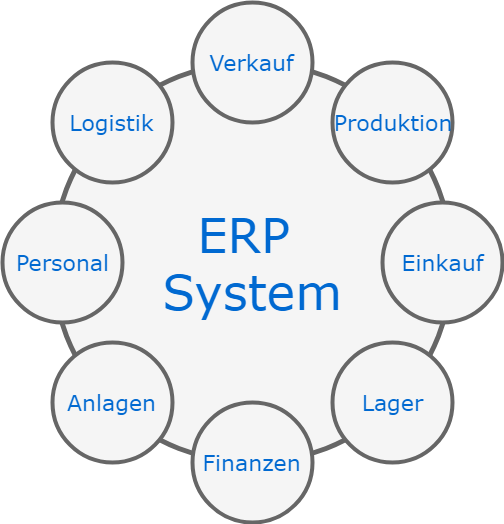
\includegraphics[width=70mm]{images/ERPModules.png}
	\caption{Schematische Darstellung: Modularisierung anhand Unternehmensabteilung}
	\label{fig:Modulisierung}
\end{figure}

Um die umfangreichen Funktionalitäten eines ERP-Systems zu gliedern und aufzuteilen, bedienen sich die meisten Hersteller eines Modul-Systems. Meist spiegelt die Aufteilung dieser Module die einzelnen Abteilungen eines Unternehmens wieder. So verteilt sich die Gesamtfunktionalität eines Systems beispielsweise auf ein Einkaufsmodul, ein Vertriebsmodul und viele andere Teilbereichsmodule auf. 
Diese Module können in ihren Grundzügen unabhängig voneinander verwendet werden. So kann ein Unternehmen beispielsweise entscheiden, vorerst nur Finanzen und Personal über das System zu verwalten. Andere Module können im Laufe der Zeit stückweise in Betrieb genommen werden. Zu den bekanntesten ERP Herstellern zählen unter anderen IBM, SAP, Microsoft, Infor und Sage.

\pagebreak
\section{Geschichte und Grundarchitektur Dynamics 365 Business Central}
\label{sec:Grundarchitektur Dynamics 365 Business Central}

\subsection{Geschichte}
\label{subsec:Geschichte}
Das ERP-System, dass heute \textit{Microsoft Dynamics 365 Business Central} heißt, erschien ursprünglich 1984 unter dem Namen \textit{PCPlus} als ein ERP System für Microsoft DOS in Dänemark\cite{DesignAndImplementationGayer}. Während seiner mittlerweile 35-jährigen Geschichte wurde das Produkt einige Male neu benannt und an den technischen Fortschritt angepasst. Was 1984 begann, wurde 1995 unter dem Namen \textit{Navision Financials} als das erste ERP-Produkt mit grafischer Benutzeroberfläche für Windows95 präsentiert. 2002 wurde \textit{Navision Financials} von Microsoft gekauft und unter dem Namen \textit{Microsoft Business Solutions Navision} vertrieben. In all diesen Jahren basierte die Datenspeicherung des Systems in einem komplexen Dateibasierten Format. Im Jahr 2008 passiert dann der Schritt zu Microsoft SQL Server und der 3-Schichten-Architektur, nun unter dem Namen \textit{Microsoft Dynamics NAV 2009}. Der vorerst letzte Meilenstein in der Geschichte des Systems ist 2018. Das System wird nun als Cloud-ERP-System unter dem Namen \textit{Microsoft Dynamics 365 Business Central} betrieben.

Trotz den vielen Versionen und der jahrzehntelangen Geschichte dieses Systems, finden sich auch in der heutigen Code-Basis noch viele Passagen, die bereits in den 1980er Jahren entstanden, und bis heute produktiv eingesetzt werden.

\subsection{3-Schichten Architektur}
\label{subsec:3-Schichten Architektur}
Dynamics 365 Business Central basiert auf einer 3-Schichten Architektur. Durch Schichtenarchitekturen lassen sich die Aufgabengebiete bzw. Teile eines komplexen Softwaresystems aufteilen. Im Falle von Dynamics Business Central 365 unterscheiden wir zwischen der Endbenutzerschicht, Serverschicht und Datenbankschicht.

\begin{figure}[h]
	\centering
	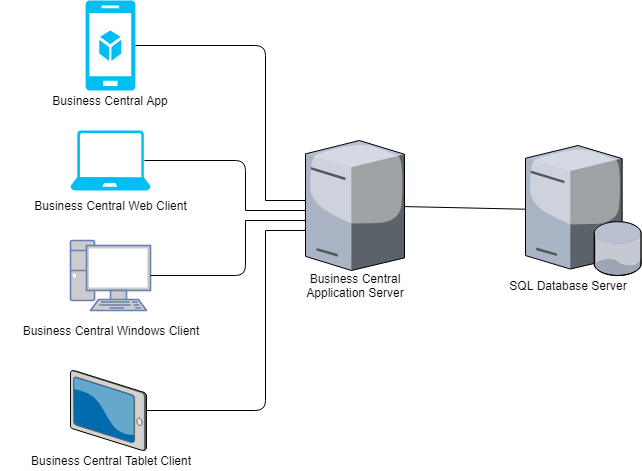
\includegraphics[width=100mm]{images/3TierArchitecture.png}
	\caption{Dynamics 365 Business Central: 3-Schichten Architektur}
	\label{fig:Image3TierArchitecture}
\end{figure}

\pagebreak

Schicht 1: Die Endbenutzerschicht/Präsentationsschicht: 
In dieser Schicht der Architektur finden sich sämtliche Softwarekomponenten, die direkt die von der Serverschicht exportierten Funktionalitäten nutzen. Hierzu zählen vorrangig die von Microsoft veröffentlichten Endbenutzerprogramme wie der Business Central WebClient und die Business Central Mobile App. Aber auch von Drittanbietern erstellte Softwarekomponenten, die Microsoft Graph API oder von Business Central veröffentlichte Webdienste nutzen sind Teil der Endbenutzerschicht.
\linebreak

Schicht 2: Die Serverschicht: 
Die Business Central Serverapplikation (auch \textit{Middle-Tier} oder \textit{Service-Tier}) stellt das Herzstück des Gesamtsystems dar. Der Business Central Server ist eine .NET basierte Serveranwendung und nutzt die Windows Communication Foundation (WCF) als Kommunikationsprotokoll. Der Server nimmt sämtliche Anfragen von Endbenutzerprogrammen entgegen, holt anhand dieser Anfragen Daten von der Datenbankschicht ab, führt mithilfe der abgeholten Daten Geschäftslogik aus, bereitet die Ergebnisse der Geschäftslogik auf, und liefert diese zurück an das anfragende Endbenutzerprogramm. Neben den Endpunkten zur Client-Kommunikation beinhaltet die Serverkomponente auch die Webserverkomponenten zur Nutzung des WebClients. Die Webserverkomponente selbst ist eine ASP.NET Core Applikation, die auf einem mitgeliefertem IIS (Internet Information Server) läuft. Daher ergibt sich auch die Anforderung, dass die Serverschicht auf einer Windows-Server Maschine betrieben werden muss.
\linebreak

Schicht 3: Die Datenbankschicht:
Hinter der Datenbankschicht verbirgt sich eine Microsoft SQL Server Instanz. Hierbei ist zu erwähnen, dass aufgrund der historischen Entwicklung des Gesamtsystems einige Funktionen einer klassischen relationalen Datenbank hier nicht verwendet werden. So wird man am Datenbankserver vergeblich nach Relationen zwischen Tabellen suchen (Fremdschlüsselbeziehung), denn diese existieren hier schlichtweg nicht. Diese Beziehungen werden von der Serverschicht verwaltet. Auf Grund dieser Tatsache ist es strengstens abzuraten manuell mit SQL Befehlen Datenbestände zu ändern. Änderungen, die nicht durch die Logik der Serverschicht validiert werden können, können schnell zu Inkonsistenzen in den Daten führen, die in weiterer Folge das Gesamtsystem korrumpieren und zu Systemausfällen führen können. 
\linebreak

Die Unterteilung der einzelnen Teilbereiche des Systems in drei Teilbereiche liefert einige Vorteile. So können anhand der vom Server exportierten Schnittstellen schnell neue Apps und 



\pagebreak
\section{Objektarten in Business Central}
\label{sec:Objektarten in Business Central}

Die Programmierung von Microsoft Dynamics 365 Business Central erfolgt durch die Erstellung und Anpassung von Applikationsbauteilen die gemeinhin \textit{Objekte} genannt werden. Diese \textit{Objekte} sind nicht mit jenen aus der klassischen objektorientierten Programmierung zu vergleichen. Dynamics 365 ist objektbasiert und nicht objektorientiert. Entwickler haben nicht die Möglichkeit neue Typen von Objekten zu erstellen, sondern nur neue Ausprägungen der bestehenden Objekttypen zu entwickeln. AL bietet gegenüber C/AL neue Möglichkeiten zur Entwicklung unter AL, was sich auch in den verfügbaren Objekttypen ausdrückt.

\begin{table}[htb]
	\centering
	\begin{tabular}{lll}
		Type           & C/AL & AL \\ 
		\\
		Table          & X    & X  \\
		TableExtension &      & X  \\
		Page           & X    & X  \\
		PageExtension  &      & X  \\
		Report         & X    & X  \\
		Codeunit       & X    & X  \\
		Query          & X    & X  \\
		XMLPort        & X    & X  \\
		MenuSuite      & X    &    \\
		Enum           &      & X  \\
	\end{tabular}
\caption{Verfügbarkeit Objekttypen: C/AL und AL}
\end{table}

Table: Tabellenobjekte definieren den Datenaufbau, Restriktionen und Validierungsregeln für alle Daten in Microsoft Dynamics 365 Business Central. Beim Kompilieren von Tabellenobjekten, veranlasst die Serverschicht die Erstellung oder Änderung einer zum Tabellenobjekt gehörigen SQL-Tabelle, in der schlussendlich die Daten landen. Tabellenobjekte sind aber weit mehr als lediglich eine Beschreibung zur Datenhaltung. Tabellenobjekte definieren auch sämtliche Validierungslogik, sowohl auf Feld- als auch auf Datensatzebene. Darüber hinaus gibt es auch die Möglichkeit, innerhalb von Tabellenobjekten Funktionen und Prozeduren für die beschriebenen Daten zu definieren.
\linebreak

TableExtension: Tabellenerweiterungen sind ein zentraler Baustein der Erweiterungsentwicklung mit AL. Sollten an einer Tabelle Änderungen oder Erweiterungen nötig sein, würde man mithilfe C/AL einfach das bestehende Tabellenobjekt abändern. Mit dem Konzept der Erweiterunsentwicklung und AL ist dies nicht mehr möglich. Genau hier kommen Tabellenerweiterungsobjekte ins Spiel. Mithilfe von Tabellenerweiterungen lassen sich Felder und Logiken eines Tabellenobjektes erweitern, ohne das Tabellenobjekt selbst zu ändern. Beim Kompilieren von Tabellenerweiterungen wird auf SQL-Seite zusätzlich zur Basistabelle eine zusätzliche hinzugefügt (textit{Companion Table}). Diese \textit{Companion Table} verfügt über den selben Primärschlüssel wie die Basistabelle, und bietet Platz für Felder der Erweiterung. Auf SQL-Seite wird für die Benennung der \textit{Companion Table} der Name der Basistabelle um die eindeutige GUID der Erweiterung ergänzt. Tabellenerweiterungen sind nur unter AL verfügbar.
\begin{figure}[h]
	\centering
	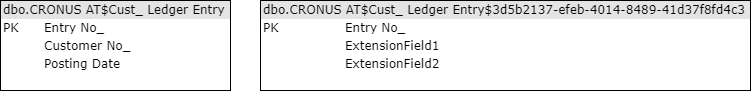
\includegraphics[width=100mm]{images/TableExtenison}
	\caption{Dynamics 365 Business Central: Standardtabelle und dazugehörige Tabellenerweiterung}
	\label{fig:TableExtension}
\end{figure}

Pages: Seiten sind unter Dynamics 365 Business Central der Baustein zur Erstellung grafischer Benutzeroberflächen. Im Vergleich zu anderen Systemen hat man hier jedoch keinen bedeutenden kreativen Freiraum bei der Gestaltung. Seiten definieren lediglich die angezeigte Information, deren Gruppierung, Sortierung und die anwendbaren Aktionen auf diese. Die visuelle Gestaltung wird bis auf wenige Ausnahmen vom System vorgegeben, sodass man als Entwickler in diesem Aspekt nur sehr eingeschränkte Möglichkeiten hat. Diese Art der Einschränkung ist zwar auf den ersten Blick als Nachteil zu betrachten, garantiert dem Nutzer des Systems jedoch ein durchgängiges Design der Benutzeroberflächen.
\linebreak

PageExtension: Mithilfe von Seitenerweiterungen lassen sich bestehende Seiten anpassen und ergänzen, ohne das ursprüngliche Seitenobjekt abzuändern. Der Benutzer merkt bei Betrachtung des Ergebnisses nicht, dass es sich hierbei um ein zusätzliches Objekt handelt. Rein optisch integrieren sich Seitenerweiterungen nahtlos in ihre Ursprungsobjekte.
\linebreak

Report: Berichte erlauben es, Auswertungen und Dokumente aus dem System zu generieren, etwa eine Bilanzübersicht, oder eine Verkaufsrechnung. Dabei bestehen Berichte aus zwei Komponenten: einem Dataset und einem Layout. Im Dataset werden die im Layout zur Verfügung stehenden Daten definiert. Das Layout selbst bestimmt die grafische Repräsentation dieser. Durch die Integration von Datasets in Microsoft Word Vorlagen, lassen sich durch den Nutzer auf einfache Weise benutzerdefinierte Word-Layouts erstellen.
\linebreak

Codeunit: Codeunits stellen die Logikkomponenten des Systems dar. Sämtliche Berechnungen, Buchungsroutinen und andere Teile der Geschätslogik finden sich hier. Um die Funktionalität einer Geschäftslogik abzuändern, ist es unter C/AL üblich direkt den verantwortlichen Code dafür abzuändern. Unter AL können bestehende Codeunits nicht geändert werden. Um unter AL Änderungen durchzuführen, müssen Event-Subscriber erstellt werden, die sich in die Standardlogik einklinken. 
\linebreak

Query: Abfrageobjekte bieten die Möglichkeit, hochperformante Abfragen an die Datenbank abzusetzen. Die Ergebnisse dieser Abfragen werden meist als Dataset für Berichte genutzt, oder als WebService exportiert.
\pagebreak

XMLPort: XMLPorts bieten eine einfache Möglichkeit, Daten in das System zu importieren und aus dem System zu exportieren. Trotz des Objektnamens, sind XMLPorts nicht nur auf XML beschränkt, sondern können auch verwendet werden um CSV und andere Formate zu verarbeiten.
\linebreak

MenuSuite: MenuSuite-Objekte bestimmen die hirarchische Menüführung des Systems, und bestimmen wie andere Objekte über die grafische Oberfläche aufgerufen werden können. MenuSuites sind nur unter C/AL verfügbar, unter AL werden die nötigen Informationen dafür direkt in den Seiten- und Reportobjekten selbst definiert.
\linebreak

Enum: Nur unter AL verfügbar. Enums definieren Aufzählungstypen und ersetzen den in C/AL verwendeten \textit{Option} Datentyp, der lediglich eine kommaseperierte Zeichenfolge darstellt, schlecht erweiterbar ist, und somit für die Erweiterungsentwicklung unter AL nicht zielführend ist.




























